%--------------------------------------------------------------------
%
%Mustervorlage fuer eine Aufgabe
%
%--------------------------------------------------------------------
%
%Ueberschreiben der automatisch erzeugten Aufgabennummer
%Die folgende Aufgabennummer ergibt sich aus dem Stand des
%Z�hlers + 1
%\setcounter{chapter}{0}
%
%
%
%
\begin{appendices}
\chapter{YDLIDAR X2 Datasheet}\label{chap:app1}

\begin{figure}[ht]
\centering
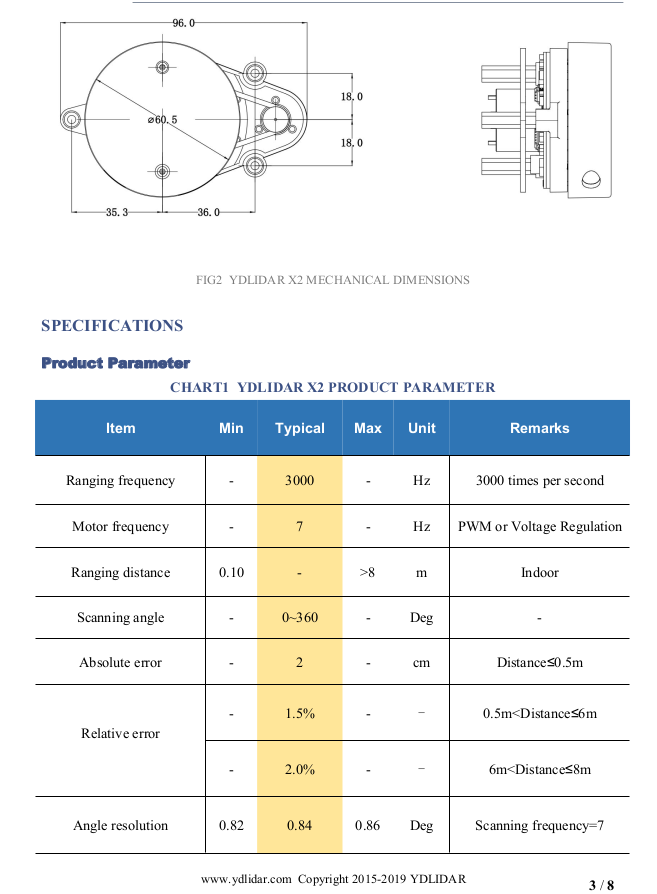
\includegraphics[width = 0.8\textwidth, frame]{./Bilder/sensorappendix.png}
\caption{YDLIDAR X2 triangulation laser scanner. \textcopyright YDLIDAR All rights reserved }
\label{ydlidar}
\end{figure}

\chapter{Directory Structure}\label{chap:app2}

\begin{figure}[ht]
\centering
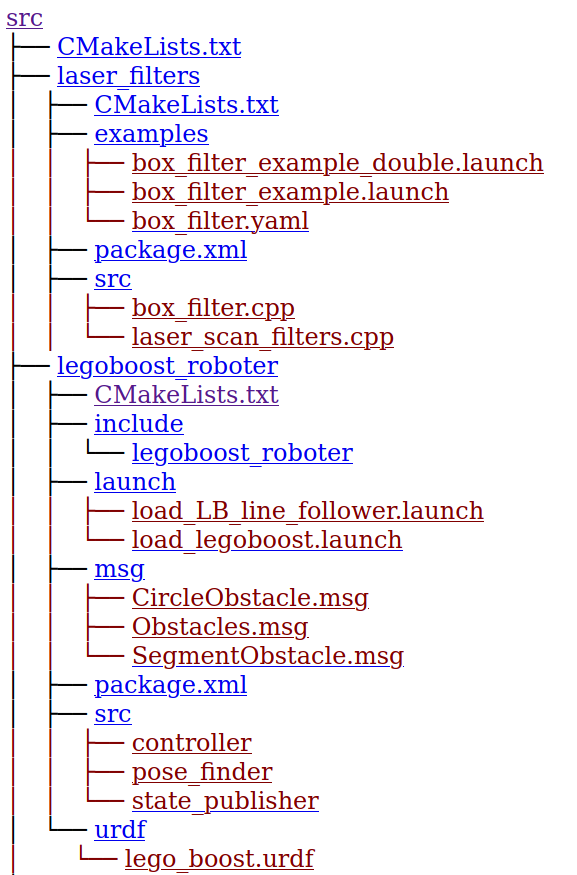
\includegraphics[width = 0.7\textwidth]{./Bilder/tree_app1.png}

\end{figure}

\begin{figure}[ht]
\centering
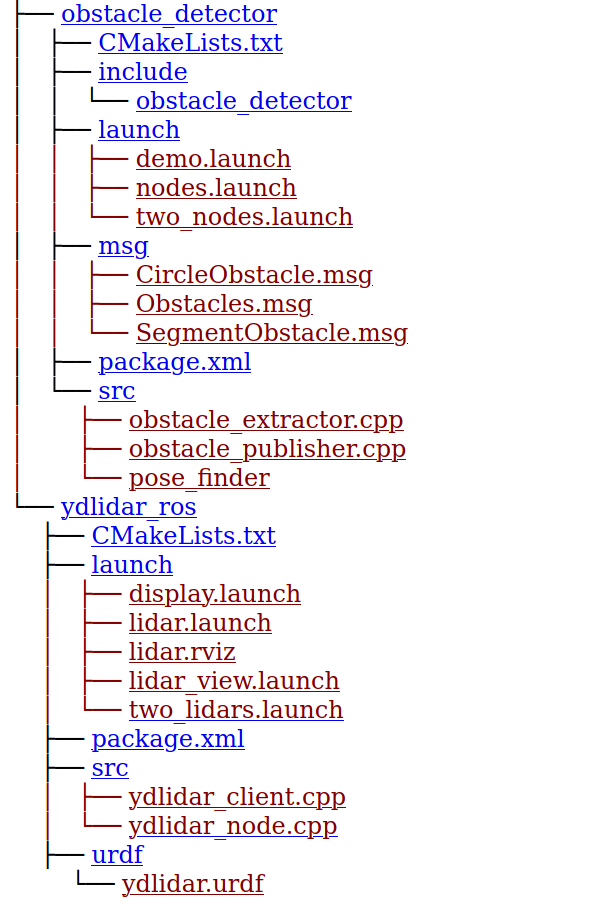
\includegraphics[width = 0.7\textwidth]{./Bilder/tree_app2.png}
\end{figure}
\end{appendices}
